\textbf{P1)} \textcolor{red}{[Prueba 1 - 2024-20]} El sistema de dos bloques de masas $M_1$ y $M_2$, junto con una polea de masa $m$ y radio $r$, se libera desde el reposo, tal como indica la figura.
Asuma que las masas de los bloques satisfacen $M_2 > M_1$  para que se produzca movimiento, y que la inercia de la polea $ I_O = \frac{mr^2}{2}. $

\begin{enumerate}[a)]
	\item  Encuentre la relación entre la rapidez angular de la polea $\omega$ y la rapidez lineal de la cuerda $v$, asumiendo que no hay deslizamiento.
	\item  Asumiendo que el bloque $M_1$ ya ha perdido contacto con la mesa, realice los DCL relevantes, incluyendo todas las fuerzas externas sobre los cuerpos.
	\item  Calcule la aceleración angular $\alpha$ y las tensiones en la cuerda.
	\item  Encuentre la velocidad de los bloques justo antes de que $M_2$ golpee la mesa.
\end{enumerate}

\center{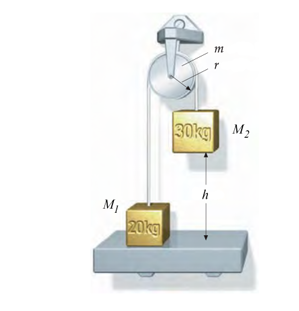
\includegraphics[width=0.5\textwidth]{imagenes/pregunta 1 ayudantia 5.PNG}}
